\documentclass[12pt,a4paper]{article}
%\usepackage[font={scriptsize,it}]{caption}
%\usepackage{relsize}
%\usepackage{float}
%\usepackage{scalerel}

\usepackage{amsmath,graphicx,amsthm,amsfonts}
\usepackage{mathtools,amssymb,bbm,cite,bm}

\theoremstyle{definition}
\newtheorem{definition}{Definition}
\theoremstyle{plain}
\newtheorem{proposition}{Proposition}
\newtheorem{theorem}{Theorem}
\newtheorem{lemma}{Lemma}
\newtheorem{corollary}{Corollary}
\theoremstyle{remark}
\newtheorem{remark}{Remark}
\newtheorem{fact}{Fact}

\setlength{\oddsidemargin}{0.1in}
\setlength{\textwidth}{6in}
\setlength{\textheight}{9in}
\setlength{\hoffset}{0in}
\setlength{\voffset}{-0.5in}

\bibliographystyle{unsrt} %unsrt or alpha

\newcommand{\Rnk}[1]{\ensuremath{\operatorname{rk}\!\left(#1\right)}}
\newcommand{\Img}[1]{\ensuremath{\operatorname{Im}\!\left(#1\right)}}
\newcommand{\Ker}[1]{\ensuremath{\operatorname{Ker}\!\left(#1\right)}}
\newcommand{\Nul}[1]{\ensuremath{\operatorname{nul}\!\left(#1\right)}}
\newcommand{\Asy}[2]{\ensuremath{\underset{#1 \to #2}{\sim}}}
\newcommand{\Pro}[1]{\ensuremath{\mathbbm{P}\!\left(#1\right)}}
\newcommand{\Tmat}[1]{\ensuremath{\matr{T}(#1)}}
\newcommand{\Smat}[1]{\ensuremath{\matr{\Sigma}(#1)}}
\DeclareMathOperator{\lcm}{lcm}
\newcommand{\vect}[1]{\bm{#1}}
\newcommand{\matr}[1]{\bm{#1}}


\begin{document}

\title{\textbf{Per-class feature importance}}

\author{Giulio Prevedello\footnote{
		Corresponding author. Electronic address: p.giulio@hotmail.it}
	\and
	Eric Cramer\footnote{
		Electronic address: cramerericm@gmail.com}
	\and
	Felice Alessio Bava\footnote{
		Electronic address: alessio.bava@gmail.com}\\ \\
}
\date{
	Institut Curie, PSL Research University,\\ CNRS UMR 3348, Orsay, France\\
	\medskip
	\today
}

\maketitle

\begin{abstract}
	Abstract\\
	\\
	\textbf{Keywords:} key1 $\cdot$ key2 \\
	\\
	\textbf{Mathematics Subject Classification:} If $\cdot$ Needed
	\end{abstract}

\section{Introduction}\label{sec:introduction}
In the past decades, the field of biology has witnessed a surge of new experimental techniques that measure hundreds of markers from thousands of cells, thus posing a challenge to analyse this multidimensional data. To analyse s a consequence, a call for new quantitative methods 

MUST DEFINE HERE X AND Y FOR THE CLASSIFICATION PROBLEM

Problem: field of biology, surge of highly multiplexed experimental protocols capable of recovering thousands of cells from which several measurements are obtained. This poses a challenge to analyse this multidimensional data. To do so, people recur to Machine Learning (ML) to identify markers that have biological relevance.

An ML method that fits the data can detect data structures that can then be challenged for biological relevance, thus helping researchers in their investigation.

Examples (Kara Davis's paper, and Garry Nolan's in general)

Feature selection is one of the desirable features. You run an experiment for several markers to classify cell types, you want to know which are the most relevant that should be retained in a follow up experiment (eventually with lower multiplexing power) to optimise the cell classification.

As cells are often classified by gating (describe gating), RF classification is an automatic routine that mimics gating. Although at present no automatic routine outperforms expert gating, thanks to the similarity with gating RF findings can be integrated, interpreted, verified with more ease from researchers.

If a ML model provides shows that an accurate prediction is achievable, it is of great interest to extrapolate which features contribute to the discrimination of one class form the others.  

There are several of these metrics, but few are backed up by theoretical results and may suffer in the case of unbalanced data.

What we seek in particular is to define a measure of that is per-class. In particular, must be robust in the case of unbalanced dataset, considering that in biology ofter rare classes (i.e. rare cell types) are of great interest.

To guide feature selection and to improve explanability in the RF classifier, we defined feature importance on a per-class basis, as a modification of the MDI feature importance (REF). This method is then applied to a classical dataset with unbalanced to illustrate the information that can be extrapolated from the RF and comparing different strategies for feature selection (REF).




[RECYCLE] In particular, the recursive thresholding in Random Forest (RF) mirrors cytometry gating to classify data, still underperfomed by automatic solution that have difficulties in dealing with biological variability while taking previous field knowledge into account.



\section{Formal definition}\label{sec:definition}
To define a measure how much each feature contributes to the prediction of one class, we follow the rationale behind the feature importance measured via mean importance decrease (MDI), which we now recall after introducing some notation as in REF.
RF is represented by a collection of decision trees (Ti)i, where each decision tree is define by a rooted binary tree graph Ti = (Vi,Ei), whose nodes either have a left and right child, otherwise are leaves. Set of leaf node DEF. 
Each node is associated to a vector v.
As the root node is associated to v $=$ all data, at each non-leaf node a decision made based on a threshold t and one of the features j so that all data in v are passed to the left child if RULE, to the right child otherwise.
For the RF, the such feature j and threshold t are determined so to maximize the impurity decrease, or gain,
delta i DEF,
where i is a measure for impurity such as the Gini or the Entropy.
Then, the variables v reaching a leaf node determines the class that is predicted in the portion of features' space identified by all the nested decisions from the nodes in the path that join the root to such leaf. IMPROVE THIS

The decision tree's importance for a given feature j, is calculated as the sum the impurity gains over all nodes, that is
EQ.
Form hereafter we refer to the vector I = Ij as global feature importance. 

We reason that, if Ij is the contribution the feature j to the overall prediction, the importance of j with respect to a class c must account for the contribution of only those nodes having at least one downstream leaf predicting class c.
must be determined by the sequence of splits that ultimately predict a portion of the space being labeled as c. Thus the feature importance relative to c accounts for the contribution of those, and only those, nodes having at least one downstream leaf assigned to the class c.

Moreover, from the perspective of a single class c, the node impurity should be affected only by the presence of variables that are not labeled to c, whichever their class. To this end, the impurity function i is replaced by the 
EQ of ic.

Finally, the per-class importance matrix, for the decision tree T, is defined as
Icj
for every class c in C and feature j in F.
ALGORITHM

Normalisation TO DO
Unbalanced data. TO DO

From equation REF, we remark that the feature importance vector relative to the class c, Ic, represents the global feature importance for the decision tree T with two classes, c and other-than-c. This property is evidenced in Figure 1 REF, which illustrates the algorithm for the per-class importance matrix, from one decision tree, as described.

In particular, being Ic is normalized in EQ REF so that the sum of its entries equals one, it is suited to represent feature importance for one class and to compare feature importance vectors between classes, in the case of imbalanced datasets.

DISEGNO

For ensemble learning methods that are defined by set of decision trees, such as RF, the importance matrix is calculated as the average of importance matrices across its trees, similarly as for the global feature importance REF.

\section{Improved explainability}\label{sec:explanability}

Explain model: heatmap and expression figures
Feature importance profile across classes -> high average for globally important features; large standard deviation for features with different impact among classes
Comparison with global importance

\section{Feature selection strategies}\label{subsec:feature_selection}
Feature importance distribution within each class
Comparison with features selected via global importance
%\begin{figure}
%	\begin{center}
%		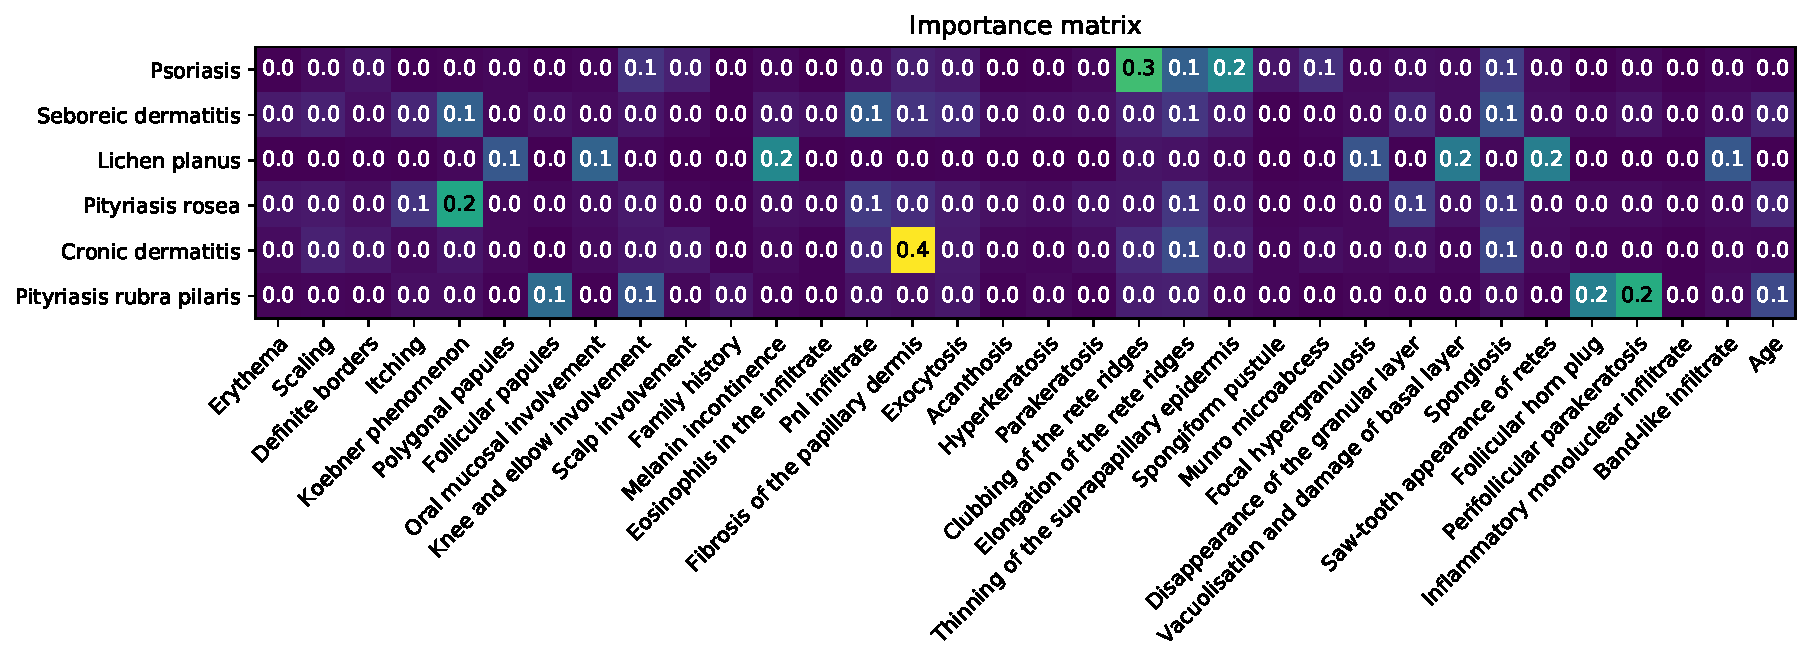
\includegraphics[width=\textwidth]{Figures/importance_matrix.pdf}
%	\end{center}
%	\caption{}\label{fig:h0_pow}
%\end{figure}

\section{Discussion}\label{sec:discussion}
Recap problem and what we achieve

\section*{Acknowledgements}
The research leading to these results has received funding from REF.
On behalf of all authors, the corresponding author states that there is no conflict of interest.

%\clearpage
\bibliography{Bibliography}


\end{document}
